\documentclass[11pt,a4paper]{letter}
\usepackage[top=0.50in, bottom=0.5in, left=1.1in, right=1.1in]{geometry}
\usepackage{graphicx}

%\signature{}

\usepackage{Sweave}
\begin{document}

\begin{letter}{}

\includegraphics[width=0.3\textwidth]{logo_uah.png}

\opening{Dear Dr. Wake:}

\noindent Please consider our paper, entitled `Phylogenetic estimates of species-level phenology improve ecological forecasting' as a Letter in \emph{Nature Climate Change.} 
. Our research addresses the critical challenge of accurately predicting the impacts of climate change on key ecosystem services and highlights the importance of incorporating phylogenetic information in ecological forecasting.
\vspace{1.5ex}\\
The current state of ecological forecasting often relies on data from a limited number of species, resulting in predictions that fail to capture the high variability observed across different species' responses. Current hierarchical models (e.g. HMM) have increased their popularity as they can deal with issues related to some species being more data-abundant than others. These models allow inference across species by pooling estimations of data-poor species towards those of more prevalent ones assuming that all species are equivalent. On the contrary, species are nested within lineages that have undergone distinct evolutionary trajectories, resulting in varied phenological responses to cues. Therefore, when estimating the data-poor species by averaging estimations from data-rich species belonging to a different lineage with entirely different phenological behavior, significant biases can occur.
\vspace{1.5ex}\\
To address this limitation, we propose an approach that extends the Phylogenetic Mixed Model (PMM) by incorporating phylogenetic structure to inform species-level sensitivities to cues. Our study demonstrates the superior performance of this new formulation compared to commonly used Hierarchical Mixed Models (HMM). Our findings reveal that species-level variability is greater than variability across cues, emphasizing the importance of accounting for phylogenetic relationships in ecological forecasting. We show that the PMM formulations outperform HMM, particularly for data-deficient species. Moreover, our approach provides insights into how different clades have evolved their phenotypes in response to multiple environmental cues operating jointly. These results have significant implications for improving ecological forecasting under changing climate scenarios beyond phenology.
\vspace{1.5ex}\\
We believe that our manuscript aligns well with the scope and objectives of \emph{Nature Climate Change}, and we have not submitted it elsewhere. We have suggested three possible reviewers (see online submission system: XX, XX2, XX3). We hope that you will find it suitable for publication, and look forward to hearing from you.
\vspace{1.5ex}\\
\noindent Sincerely,\\
\vspace{1.5ex}\\
 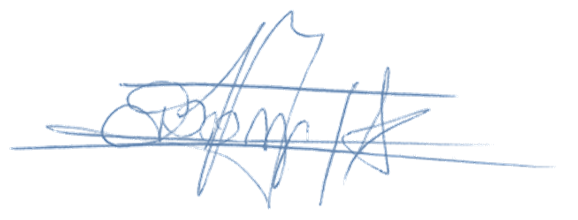
\includegraphics[width=0.2\textwidth]{Signature_IMC.png} \\
 \vspace{1.5ex}\\
\noindent Ignacio Morales-Castilla


\end{letter}
\end{document}
